\documentclass{beamer}

\usepackage[utf8]{inputenc}
\usepackage{svg}
\usepackage{graphicx}
\usepackage{lmodern}

\usetheme{AnnArbor}
\usecolortheme{beaver}

\begin{document}

\title{Bioinformatics of the Immune System}
\author{Lasath Fernando}

\begin{frame}
\titlepage
\end{frame}

\section{Background}
\subsection{Immune Response}
\begin{frame}
  \frametitle{Immunoglobulins}

  \begin{columns}
    \begin{column}{5cm}
    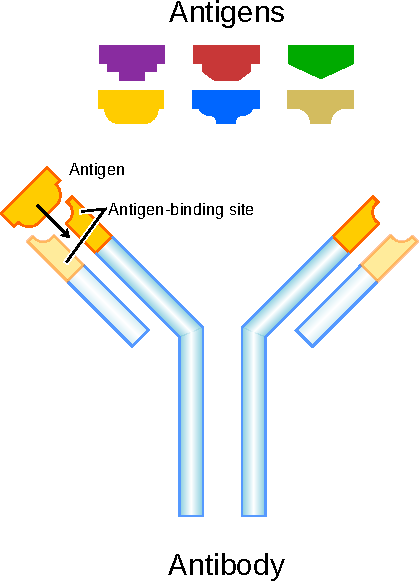
\includegraphics[width=\textwidth]{antibody.pdf}
    \end{column}
    \begin{column}{5cm}
    \begin{itemize}
     \item Also known as antibodies
     \item Y-shaped protien
     \item Binds to a very specific antigen, which is doomed from that point.
     \item Needs to be extremely specific as a result.
     \item Produced by B-Cells
    \end{itemize}

    \end{column}
  \end{columns}

\end{frame}

\begin{frame}
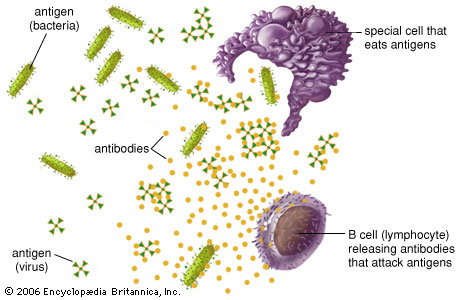
\includegraphics[width=\textwidth]{antigens-antibodies.jpg}
\end{frame}

\begin{frame}
\frametitle{B-Cell}
\begin{columns}
  \begin{column}{.5\textwidth} 
    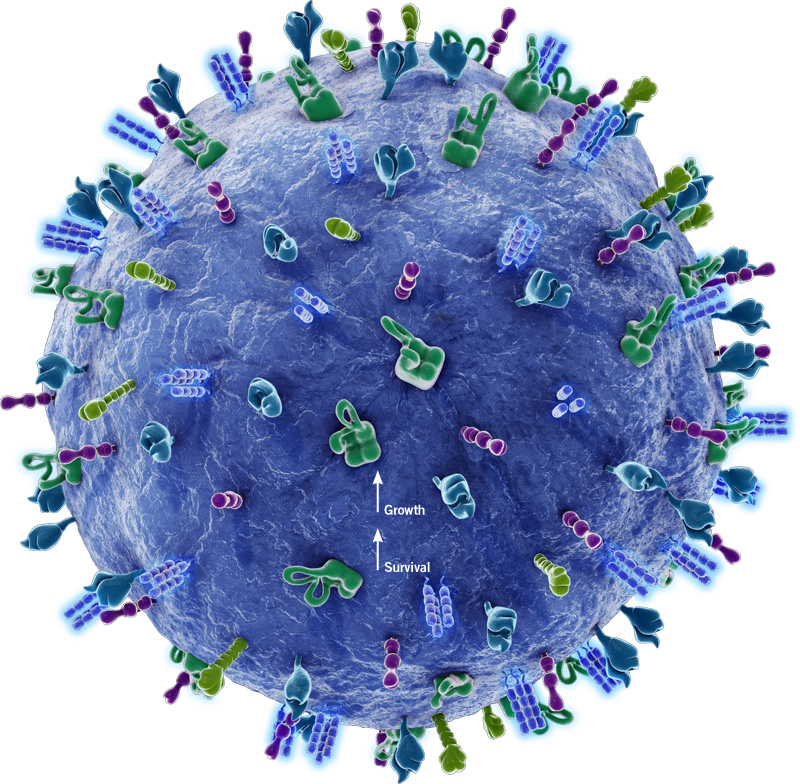
\includegraphics[width=\textwidth]{b-cell.jpg}
  \end{column}
  \begin{column}{.5\textwidth} 
    \begin{itemize}
     \item Produces a particular antibody
     \item Some of them dettach and float around on their own
     \item Contains the rearranged (mutated) DNA
    \end{itemize}
  \end{column}
\end{columns}
\end{frame}

\subsection{Combination Process}

\begin{frame}
\frametitle{Combination Process}
\begin{columns}
  \begin{column}{.5\textwidth} 
    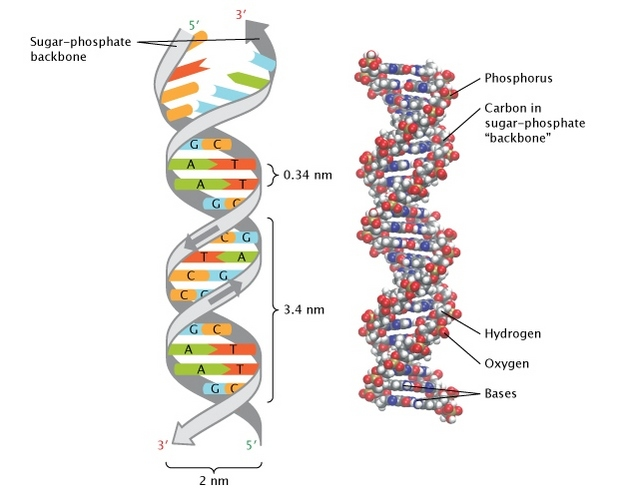
\includegraphics[width=\textwidth]{dna-strand.jpg}
  \end{column}
  \begin{column}{.5\textwidth} 
    \begin{itemize}
      \item Not fully understood
      \item Immunoglobulin consist of 2 heavy chains, and 2 light chains.
      \item IGHV, IGHD and IGHJ genes.
    \end{itemize}
  \end{column}
\end{columns}
\end{frame}

\subsection{Machine Learning}

\begin{frame}
\frametitle{Hidden Markov Model}
\begin{columns}
  \begin{column}{.5\textwidth} 
  %%TODO: find HMM pic
    \includegraphics[width=\textwidth]{}
  \end{column}
  \begin{column}{.5\textwidth} 
    \begin{itemize}
      \item Commonly used in machine learning for speech recognition
    \end{itemize}
  \end{column}
\end{columns}
\end{frame}

\section{Motivation}

\subsection{IHMMuneAlign}

\begin{frame}
\frametitle{IHMMuneAlign}
\begin{itemize}
 \item Is given the rearranged gene sequence that's found in the B-Cell (For a particular Immunoglobulin).
 \item Attempts to determine the sequences that formed it
 \item Represents the known steps of the recombination process as states in a HMM.
 \item Runs viterbi algorithm to determine the chain of states that caused the observations (The rearranged sequence)
\end{itemize}
\end{frame}

%%TODO: Mention increasing data sets (100,000 genes)

\section{Plan}
\begin{frame}
\frametitle{Existing Implementation}
\begin{itemize}
 \item Written in Java
 \item Uses BioJava
 \item Was designed for single run
 \item Does iteration in launcher script
 \begin{itemize}
  \item Overhead of spinning up/tearing down JVM after each one
  \item Reading data files each time
  \item Invaliding caches/buffers etc
 \end{itemize}

\end{itemize}


\end{frame}

\end{document}
